% Chapter 1

\chapter{Estado del arte} % Main chapter title

\label{Chapter2} % For referencing the chapter elsewhere, use \ref{Chapter1}



\section{Conservación de procedimiento científicos}

Distintas áreas de la ciencia han adoptado técnicas y herramientas para conservar el procedimiento. Por ejemplo, investigadores en bio-informática ha incorporado los workflows para distintos análisis: 
Doblamiento de proteínas \cite{craddock2006science}, secuencias de DNA y RNA \cite{blankenberg2010galaxy,giardine2005galaxy} y la detección de ondas gravitacionales \cite{deelman2004pegasus}.
Los workflows científicos son métodos que permiten representar un conjunto de pasos computacionales. Estos pasos pueden ser la obtención de los datos de entrada, transformaciones o generación de los resultados.
La representación de los workflow se construye en un lenguaje abstracto para simplificar la complejidad. El conjunto de pasos se pueden representar como gráfos sin ciclos y dirigidos, donde cada paso computacional es representado por un nodo y las dependencias entre los pasos son representado por los arcos.
El uso de sistemas de manejo de workflows científicos \textit{Scientific Workflow management Systems (WMS)} permiten diseñar abstractamente, ejecutar y compartir el procedimiento científicos. 

Dado que los workflows formalmente describen la secuencia de tareas computacionales y administración de datos, es fácil encontrar el camino de los datos producidos.
Un científico podría ver el workflow y los datos, seguir los pasos y llegar al mismo resultado. En otras palabras, la representación del workflow facilita la creación y administración de la computación y además construye una base en la cual los resultados pueden ser validados y compartidos.

Sin embargo, múltiples estudios han mostrado las dificultades reproducir los resultados de los experimentos.

%todo: ampliar estos


%Como se menciono, la mayoría de las propuestas de reproducibilidad de ambientes en las ciencias de computación se han enfocado en los datos, el código y la descripción de workflow pero ha dejando de lado los recursos computacionales y componentes de software. Siendo un recurso esencial para reproducir el experimento

%De acuerdo a \cite{king1995replication}, en orden de reproducir o replicar un artefacto digital es necesario manejar su conservación y para alcanzar esta conservación se debe garantizar que: existe la suficiente información con la cual se pueda entender, evaluar y construir un trabajo anterior sin información adicional del autor. 

%Uno de los trabajos que se ha enfocado en conservar los recursos de un ambiente computacional es \cite{santana2017reproducibility}. Donde los autores han identificado dos enfoques para conservar un ambiente científico. Conversación física: donde el objeto real es conservado dada la relevancia y la dificultada de obtener una replica y  Conversación lógica: donde los objetos son descriptos en una manera que un experimento similar puede ser obtenido en un futuro experimento.


\subsection{Sistemas de administración de workflows}

Cómo se menciono anteriormente, los workflows científicos permiten a los usuarios expresar fácilmente tareas computacionales de varios pasos, por ejemplo, recuperar datos de un instrumento o una base de datos, reformatear los datos y ejecutar un análisis. 
Un workflow científico describe las dependencias entre las tareas y la mayoría de los casos se describe como un gráfico acíclico dirigido (DAG), donde los nodos son tareas y los bordes denotan las dependencias de las tareas.
Una propiedad que define un workflow científico es que gestiona el flujo de datos. Es por ello, que las tareas en un  workflow científico varían ampliamente según las necesidades del autor, los tipos pueden ser tanto como tareas cortas en serie o tareas paralelas muy grandes (e.g, utilizando Message Passing Interface - MPI) rodeadas de un gran número de pequeñas tareas en serie utilizadas para el pre y post procesamiento.
La interpretación y ejecución de los workflows son manejados por un sistema de manejo de workflows (WMS) que administra la ejecución de la aplicación en la infraestructura. 
Un WMS puede ser considerado como una capa intermedia necesaria para la abstracción y orquestación de prodecimiento científico. A continuación se describe algunos de los WMS más populares.

Actualmente, existen múltiples WMS que han sido generado por diversas comunidades.

\begin{description}
	\item [Galaxy:] Galaxy (Goecks et al., 2010) is a web-based WMS that aims to bring computational data analysis capabilities to non-expert users in the biological sciences domain. The main goals of the Galaxy framework are accessibility to biological computational capabilities and reproducibility of the analysis result by tracking the information related to every step on the process. 
	\item [Taverna: ] Taverna is a Web Service-based WMS, as all the components of the workflow must be implemented as web services (either locally or using an available remote service). Taverna is able to integrate Soaplab26, REST (Fielding, 2000) and WSDL (Christensen et al., 2001) web services. It offers a wide range of services for different processing capabilities, such as local Java services, statistical R processor services, XPath scripts, or spreadsheet import services.
	\item [Pegasus:] Pegasus (Deelman et al., 2005) is a WMS able to manage workflows comprised of mil- lions of tasks, recording data about the execution and intermediate results. In Pegasus, workflows are described as abstract workflows, which do not contain resource informa- tion, or the physical locations of data and executables.
	\item [WINGS:] WINGS (Gil et al., 2011) may not be considered as a proper WMS by itself, as it does not provide workflow enactment and execution features. However it is widely known for workflow design. WINGS can be seen as a top-level and domain-oriented design tool whose workflows can be later enacted in different workflow engines, such as Pegasus or Apache OODT29.
	\item [dispel4py:] dispel4py (Filguiera et al., 2014) is a Python (Rossum, 1995) library for describing workflows. It describes abstract workflows for data-intensive applications, which are later translated and enacted in distributed platforms (e.g. Apache Storm, MPI clusters, etc.).

\end{description} 



\section{Conservación de equipamiento}
Comúnmente el equipamiento en otras disciplinas no es un problema a resolver dado que los recursos utilizados son son conocidos, no-variables y estándares. Por ejemplo, la utilización de probetas, microscopios u otros elementos físicos. 
Consecuentemente, los investigadores pueden nombrarlos e identificarlos de forma manual en los procedimientos de sus cuadernos de laboratorio. Lo que permite que otro investigador conozca cuáles fueron las herramientas utilizadas en el experimento.
Aunque existen excepciones como en la ciencia de biología, donde ciertos recursos son materiales que son utilizados en los procedimientos. En estos casos, los investigadores deben describir los materiales incluyendo información como marcas, composición y otros. 
En otras ciencias como la astronomía se utilizan recursos  de alta tecnología, donde también es necesario documentar las características de hardware y configuraciones utilizadas en el proceso experimental. 
En las ciencias de la computación sucede un caso similar, dado que los recursos computacionales son una componente requerida en la ejecución del sistema. 
Es por ello, que esta comunidad no puede ser la excepción respecto a la descripción de los recursos. Por lo tanto, los autores deben poder documentar computadores, clusters, servicios web, componentes de software, etc., en el contexto de sus experimentos.

Diversos trabajos han estudiado el estado actual de la reproducibilidad en las ciencias de computación, en \cite{DBLP:conf/eScience/ZhaoGBKGGHRRG12} se estudia el factor de decaimiento de un conjunto workflows científicos almacenado en myExperiment \footnote{\url{https://www.myexperiment.org/home}} que fueron diseñados para el WMS Taverna \cite{DBLP:journals/bioinformatics/OinnAFMSGCGPWL04} del área de biología. Para ello, los autores utilizaron cuatro conjuntos de paquetes de workflows y clasifican el decaimiento de los workflows en cuatro categorías: recursos de terceros volatiles, datos de ejemplos faltantes, ambiente de ejecución faltante y descripciones insuficientes sobre los workflow. El estudio muestra que casi el 80\% de workflows fallan al ser reproducidos, con un 12\% de esos fallos debido al ambiente de ejecución faltante y 50\% recursos de terceros volatiles. Estas dos últimas categorías están asociadas a la conservación del ambiente computacional del experimento.
En \cite{DBLP:conf/ipres/MatthewsCWJBS09}, los autores describen un procedimiento para preservar el software, argumentando que el software es frágil a los cambios de ambiente ya sea hardware, sistema operativo, versiones de las dependencias y configuración. Los autores afirman que el software no puede ser preservado con la metodología anterior de sólo mantener su código binario ejecutable. Por ello, introducen el concepto de adecuación de la preservación, una métrica para medir si la preservación de conjunto de funcionalidades de componente de software luego de un proceso reproducción.

De la misma manera, editoriales se ha enfocado en intentar resolver los desafíos en la publicación de trabajos científicos. Por ejemplo, Elsevier formó el \textit{Executable Paper Grand Challenge} para abordar la dificultad de reproducibilidad de los resultados en las ciencias de la computación, ellos  argumentan que los bloques vitales y necesarios de información para replicar los resultados -por ejemplo, software, código, grandes conjuntos de datos- no suelen estar disponibles en el contexto de una publicación académica. 
Y \textit{Executable Paper Grand Challenge} creó una oportunidad para que los científicos diseñen soluciones que capturen esta información y proporcionen una plataforma para que estos datos puedan ser verificados y manipulados. 
En 2011, \cite{DBLP:journals/procedia/BrammerCMW11} se argumenta que el documento de investigación en su estado actual ya no es suficiente para reproducir, validar o revisar completamente los resultados y conclusiones experimentales de un documento. Esto impide el progreso científico. 
Para remediar estas preocupaciones, presentan Paper Mâché, un nuevo sistema para crear documentos de investigación dinámicos y ejecutables. La principal novedad de Paper Mâché es el uso de máquinas virtuales, que permite a los lectores y revisores ver e interactuar fácilmente con un documento y poder reproducir los principales resultados experimentales.
En la misma línea, CernVM \cite{buncic2010cernvm} propuso la utilización de máquinas virtuales para resolver problemas de reproducibilidad en la ciencia. CernVM es un sistema para el uso de máquina virtuales capaz de ejecutar aplicaciones físicas de los experimentos relacionados al \textit{Large Hadron Collider} (LHC) en el \textit{European Organization for Nuclear Research} (CERN). Su objetivo es proporcionar un entorno completo y portátil para desarrollar y ejecutar el análisis de datos LHC en cualquier ordenador del usuario final (portátil, de sobremesa), así como en la red, independientemente de las plataformas de sistemas operativos (Linux, Windows, MacOS). La motivación del uso de técnicas de virtualización que permite separar los recursos de computación desde la infraestructura subyacente.

Algunos autores han expuesto la necesidad de capturar y preservar el entorno de ejecución de un ejecución del experimento, proporcionando herramientas para analizar y empaquetar los recursos involucrados en él.
ReproZip \cite{DBLP:conf/tapp/ChirigatiSF13} busca captar el conocimiento sobre una infraestructura e intentar reproducirla en un nuevo entorno. Esta herramienta lee los componentes de infraestructura involucrados en la ejecución (archivos, variables de entorno, etc.) y almacena esta información en una base de datos MongoDB \footnote{\url{https://www.mongodb.com/es}}. 
A continuación se recogen y empaquetan los elementos descritos. Luego, el sistema debe desempaquetar los elementos  en otra máquina para reproducir el experimento. Sin embargo, este tipo de enfoque que empaqueta los componentes físicos de una infraestructura determinada presenta limitación en la práctica, debido que los paquetes deben ser ejecutado en una máquina destino similar.
Otro ejemplo es TOSCA (Topology and Orchestration Specification for Cloud Applications), TOSCA es un ejemplo de las soluciones que han definido sintaxis para describir la ejecución de los ambientes computacionales. TOSCA es un lenguaje de código abierto utilizado para describir las relaciones y dependencias entre servicios y aplicaciones que residen en una plataforma de computación. TOSCA puede describir un servicio de computación en nube y sus componentes y documentar la forma en que están organizados y el proceso de orquestación necesario para utilizar o modificar dichos componentes y servicios. Esto proporciona a los administradores una forma común de gestionar aplicaciones y servicios en la nube, de modo que esas aplicaciones y servicios puedan ser portátiles a través de las diferentes plataformas de los proveedores de cloud computing. 
Otro esfuerzo importante relacionado a nuestro trabajo incluye la descripción de los ambientes computaciones utilizando ontologías es TIMBUS. El proyecto se focaliza en preservar procesos de negocios y su infraestructura computacional.  Para ello, propusieron un extractor para extraer y anotar los componentes de Software y Hardware, éstas anotaciones son almacenadas según un conjunto de ontologías con el objetivo de gestionar la preservación y reejecución de los procesos de negocio. Sin embargo, el enfoque extractor del Proyecto Timbus no es adecuado para ser utilizado en cualquier sistema de virtualizada ya que aumenta la complejidad del ambiente y generando ruido. Además, exige ejecutar el ambiente computacional lo cual conlleva altos costos computacionales, disminución en la escalabilidad y creación de brechas de seguridad. 

En el enfoque de describir los recursos computacionales, los autores en \cite{santana2017reproducibility} identificaron dos enfoques para conservar el  ambiente computacional de un experimento científico: la conservación física, donde los objetos de investigación dentro del experimento se conservan en un entorno virtual; y la conservación lógica, donde las principales capacidades de los recursos en el entorno se describen utilizando vocabularios semánticos para permitir al investigador reproducir un entorno equivalente. Para ello, definieron un proceso para documentar la aplicación de flujo de trabajo y su sistema de gestión relacionado, así como sus dependencias. Además, los autores propusieron \textit{The Workflow Infrastructure Conservation Using Semantics ontology} (WICUS). WICUS es una red de ontologías OWL2 (Web Ontology Language) que implementan la conceptualización de los principales dominios de una infraestructura computacional. Como: Hardware, Software, Workflow y Recursos Informáticos. 
Los autores argumentan este trabajo debido que a que el workflow científico requiere un conjunto de componentes de software, y los investigadores deben saber cómo desplegar esta pila de software para lograr un entorno equivalente.
Sin embargo, este proceso se realiza de forma de manual, dejando mucho trabajo a los científicos. 
Además, los autores afirman que la conservación de los ambientes computacionales comúnmente se logra utilizando un enfoque físico dado que la conservación física permite compartir fácilmente un ambiente computacional con otros investigadores y ellos pueden reproducir el experimento utilizando en el mismo ambiente. 
Sin embargo, los esfuerzos necesarios para mantener la infraestructura son altos y no hay garantías que no sufran un proceso de decaimiento \cite{DBLP:journals/fgcs/DeelmanVJRCMMCS15}.  
Consecuentemente, la mayoría de los trabajos dejan fuera del ámbito de aplicación la conservación física del entorno informático del workflow (basándose en la infraestructura elegida). Pese a que la conservación lógica y física son deseadas para lograr la reproducibilidad del experimento. 

En diversos trabajos ~\cite{DBLP:journals/bioinformatics/LeprevostGARUBV17, Beaulieu2017, Boettiger:2015:IDR:2723872.2723882, aranguren2015enhanced} se ha propuesto la utilización de Docker como un reemplazo al uso de máquinas virtuales como ambiente computacionales científicos, los trabajos argumentan que Docker presenta beneficios de portabilidad, documentación precisa de la instalación y configuración, manejo de control de versiones de las imágenes y fácil adopción por desarroladores. 
Un ejemplo de uso de Docker para la reproducibilidad es BioContainers \cite{DBLP:journals/bioinformatics/LeprevostGARUBV17}. BioContainers es un framework de código abierto y orientado a la comunidad que proporciona entornos ejecutables independientes de la plataforma para el software de bioinformática. BioContainers permite a los laboratorios instalar fácilmente software de bioinformática, mantener múltiples versiones del mismo software y combinar herramientas de análisis. BioContainers se basa en los populares proyectos de código abierto Docker~\footnote{\url{https://www.docker.com/}}, Singularity~\footnote{\url{https://www.sylabs.io/singularity/}} y rkt~\footnote{\url{https://coreos.com/rkt/}}, que permiten que el software sea instalado y ejecutado bajo un entorno aislado y controlado.
Sin embargo, en \cite{Boettiger:2015:IDR:2723872.2723882,DBLP:conf/semweb/OsorioAV18} los autores exponen que Docker no controla que paquetes instalados en las imágenes y no existe una descripción completa de los componentes de la imagen y consecuente del contenedor. Por lo tanto, las imágenes Docker funcionan como una caja negra, lo que significa que los usuarios saben cuál es el paquete que se ejecuta dentro del contenedor pero no conocen las versiones o los otros paquetes necesarios para ejecutarlo.

Respecto a la descripción de los componentes de una imagen Docker, en \cite{Shu:2017:SSV:3029806.3029832:DockerHub:Security} analizó más de 300.000 imágenes de Docker almacenadas en el repositorio oficial de Docker. Los autores encontraron que en promedio las imágenes que contiene el Docker Hub (sistema de almacenamiento de imágenes) son más de 180 vulnerabilidades, siendo la raíz de tal cantidad de vulnerabilidades el hecho de que muchas imágenes no han sido actualizadas en varios días y que muchas de estas vulnerabilidades se propagan de imágenes de padres a hijos. Los autores encontraron correlaciones entre las imágenes más influyentes y los paquetes vulnerables mejor clasificados, lo que sugiere que la fuente de esa cantidad de vulnerabilidades era probablemente el resultado de la propagación de un pequeño número de imágenes populares (debido a la falta de actualización de las imágenes principales). Los autores utilizaron el software Clair \footnote{\url{https://github.com/coreos/clair}} de la empresa CoreOS\footnote{\url{https://coreos.com/}}. 
En términos de ingeniería ontológica, los autores en~\cite{huo2015smart} presentan la ontología Smart Container que extiende DOLCE~\cite{gangemi2002sweetening} y modela Docker en términos de sus interacciones para desplegar imágenes. Otro trabajo relacionado, ~\cite{tommasini2017representing}  describe cómo usar RDF para representar archivos de construcción de Docker. 

\section{Docker}

	Durante los años el uso de tecnologías de virtualización ha aumentado
	rápidamente, esta tecnología permite dividir el sistema de un computador
	en múltiples ambientes virtuales. Los importantes beneficios que entrega esta
	tecnología ha hecho que la virtualización sea muy utilizada \cite{bui2015analysis}.
	Uno de los usos comunes para esta tecnología es la virtualización de 
	servidores en \textit{datacenters}. Con la virtualización de servidores, un
	administrador de sistemas puede crear una o más instancias virtuales o 
	máquinas virtuales (VMs) en un servidor y hoy en día se utiliza comúnmente en
	\textit{datacenters} y también en plataformas de \textit{cloud} como Amazon
	EC2, RackSpace, Dreamhost y otros \cite{felter2014updated}. El crecimiento
	el uso de la virtualización ha hecho necesario la búsqueda de una solución
	que permita tener un ambiente escalable y seguro. Un gran numero de
	soluciones han nacido en el mercado y se pueden clasificar en dos tipos:
	\textit{container-based virtualization} y \textit{Virtualización basada en hipervisores}.

	\textit{Container-based virtualization} es una virtualización liviana a
	nivel de software usando el kernel de host para correr múltiples ambientes.
	Estos ambientes son nombrados con \textit{containers} (contenedores).
	Hoy en día Linux-VServer, OpenVZ, libcontainer y Linux Container (LXC) son
	las principales implementaciones para utilizar contenedores. En la
	figura~\ref{fig:container-arch} se puede observar que la arquitectura de
	\textit{container-based virtualization}  que trabaja con un sistema
	operativo compartido con el host por lo tanto no es necesario cargar \(n\) veces el sistema
	operativo por \(n\) containers. Para el sistema operativo \textit{host} el
	\textit{container} es un proceso más que corre encima del kernel. Gracias al
	kernel y otras herramientas proveen un ambiente aislado con los recursos limitados
	necesarios para ejecutar las aplicaciones en el \textit{container} \cite{merkel2014docker}.
	
	\begin{figure}[]
  		\centering
    	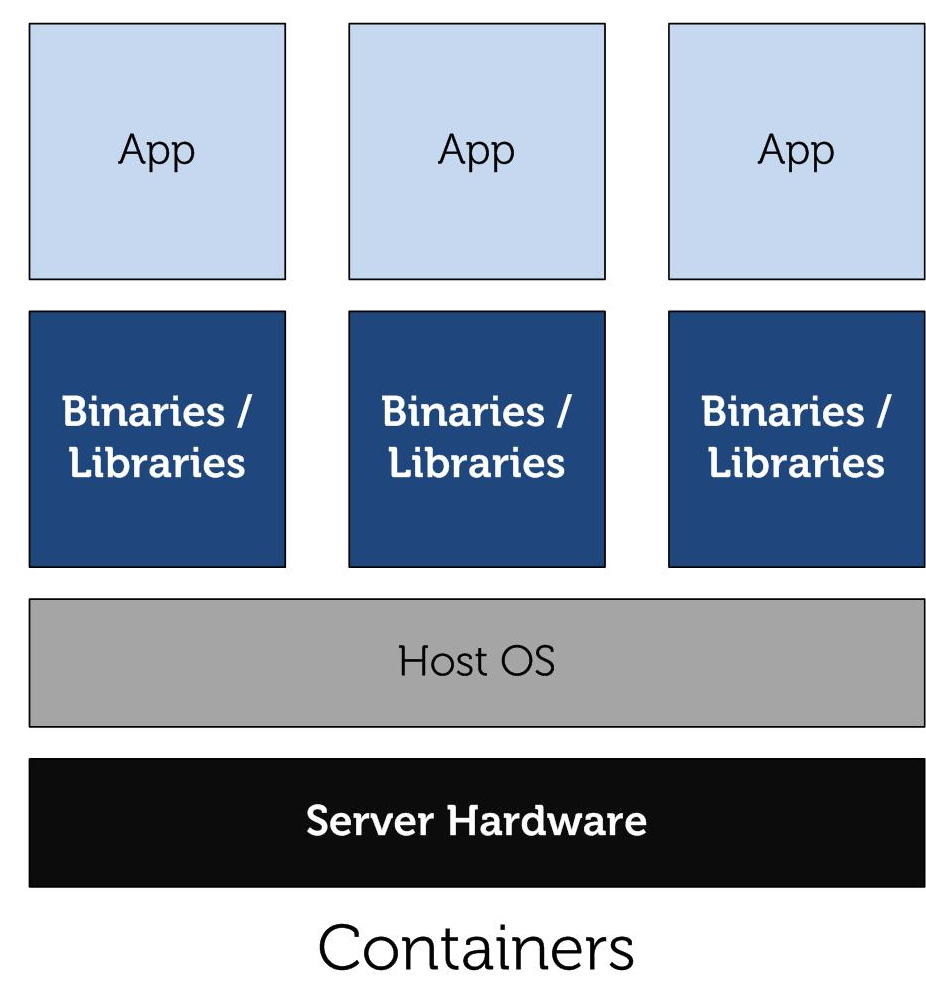
\includegraphics[width=0.35\textwidth]{Figures/containers.png}
    	\caption{Container-based virtualization.}
    	\label{fig:container-arch}
	\end{figure}
	Por otra parte \textit{hypervisor-based} establece una máquina virtual (\textit{virtual
	machine})   encima del sistema operativo, cada máquina virtual (VM) no solamente
	incluye la aplicación y las dependencias sino además incluye el sistema 
	operativo completo con otro kernel separado.

	\begin{figure}[]
 		\centering
    	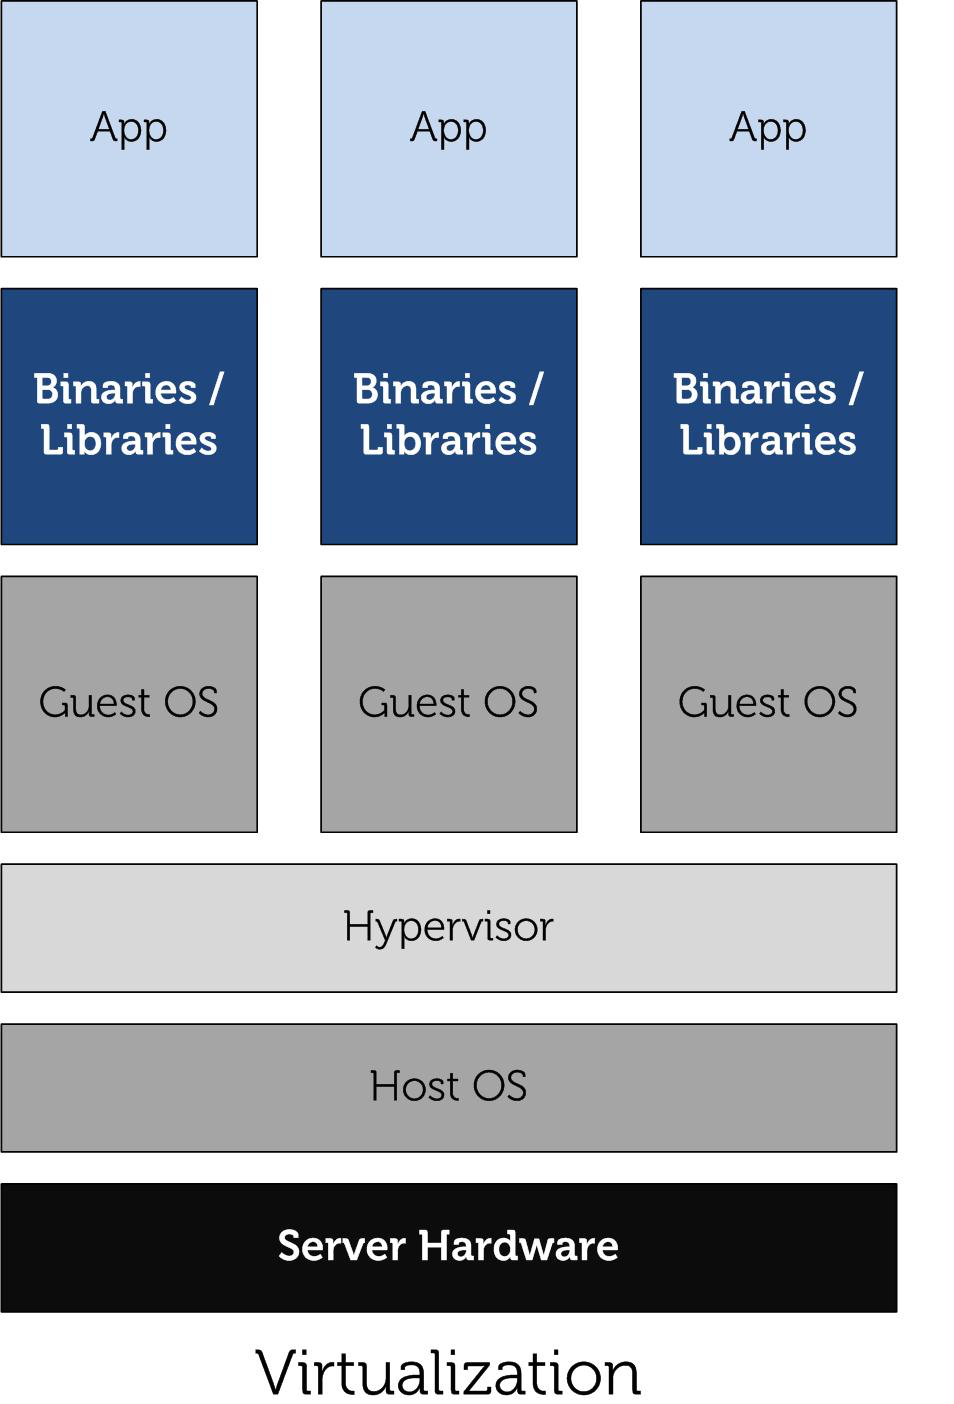
\includegraphics[width=0.3\textwidth]{Figures/virtual.png}
    	\caption{Hypervisor-based virtualization.}
    	\label{fig:vm-arch}
	\end{figure}
	Las diferencias entre estos dos tipos de virtualización presenta ventajas interesantes para
	\textit{container-based virtualization} como una mayor densidad de ambientes
	virtuales en un host debido a que no debe cargar el sistema operativo y puede
	compartir los binarios y bibliotecas con otros containers en el mismo host.
	Segundo se ha demostrado que la \textit{container virtualization} es capaz de
	ser más liviana y eficiente \cite{padala2007performance,regola2010recommendations,felter2014updated}. A partir de esto nace la motivación de estudiar más a fondo soluciones que utilicen los containers y la seguridad de estos. \\


Docker es un proyecto open-source que utiliza la tecnología de los containers (libcontainer) para ``construir, migrar y correr aplicaciones distribuidas". Actualmente utilizado por Yelp, Spotify, entre otros \cite{Docker:2015:Online, marmolnetworking}
Docker es una solución que simplifica el uso de los \textit{containers} que han estado presente durante más de una década. Primero provee una interfaz simple y segura para crear y controlar \textit{containers} \cite{bui2015analysis}, segundo permite a los desarrolladores empaquetar y correr sus aplicaciones de manera sencilla y además se integra con herramientas terceras que permiten administración y despliegue como Puppet, Ansible y Vagrant. Además que existen diversas herramientas de orquestación como Mesos \cite{Apach91:online}, Shipyard \cite{shipy13:online}, Kubernetes \cite{kubernetes:2015:Online}, RancherOS \cite{Ranch38:online} y Docker Swarm	 \cite{Docke38:online}.
  Docker puede separarse en dos grandes componentes: 
  
  	Dentro de Docker Engine existen  componentes: 
	\begin{itemize}
		\item Docker Engine
		\item Docker Images
		\item Docker Containers
		\item Docker Registries
	\end{itemize}
	

Docker Engine es una herramienta liviana y portable para manejar \textit{container-based virtualization} utilizando la arquitectura de la figura \ref{fig:docker}. Los containers corren encima del servicio de Docker que se encarga de ejecutar y manejar los \textit{containers}. Docker Client, provee una interfaz para interactuar con los containers con los usuarios a través de RESTful APIs\cite{bui2015analysis}.\\

\begin{figure}[]
  \centering
    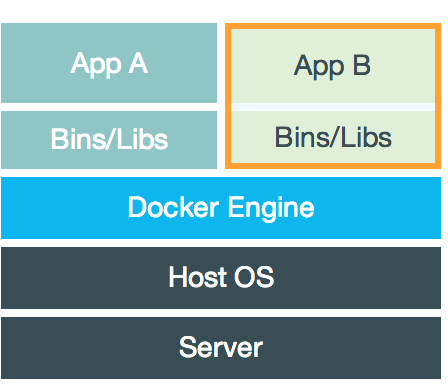
\includegraphics[width=0.3\textwidth]{Figures/docker.png}
    \caption{Docker}
    \label{fig:docker}
\end{figure}

	Docker utiliza una arquitectura de cliente-servidor, Docker Client habla con Docker Daemon y este construye, maneja y corre los \textit{containers}. Docker Client y Docker Daemon pueden correr en el mismo host o se puede conectar el cliente desde un host remoto. El cliente y el Daemon se comunican en forma de sockets o RESTful API \cite{Docker:2015:understanding}.
	
\begin{figure}[]
  \centering
    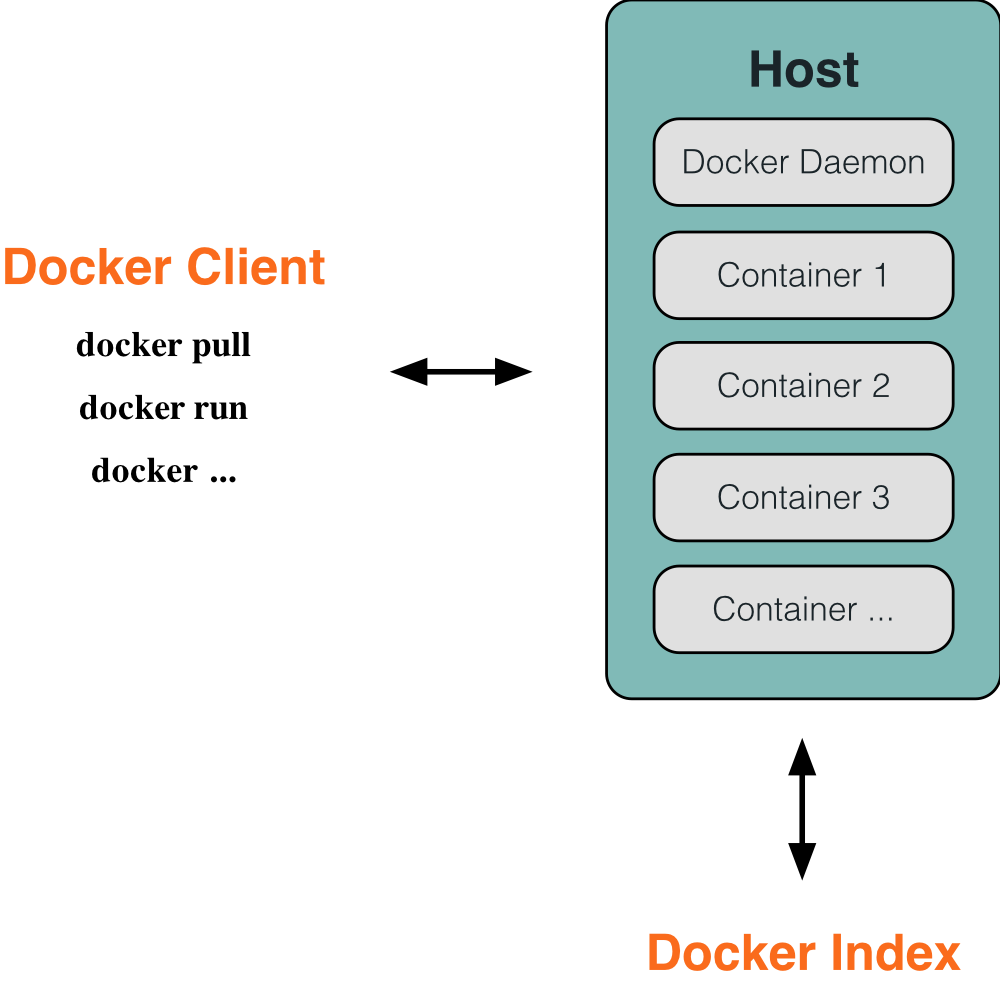
\includegraphics[width=0.3\textwidth]{Figures/architecture.png}
    \caption{Arquitectura}
    \label{fig:arquitectura}
\end{figure}	
	

	Una imagen de Docker (\textit{Docker Image}) es una plantilla de solo lectura (\textit{read-only template}). Por ejemplo, una imagen puede contener un sistema operativo de Ubuntu con Apache y una aplicación web instalada o simplemente el sistema operativo. Las imágenes son usadas para construir \emph{Docker containers}. Cuando el usuario crea cambios en el \textit{container}, este cambio no se realiza en la imagen, sino  que Docker añade una capa adicional con los cambios de la imagen\cite{bui2015analysis}. Por ejemplo, si el usuario utiliza una imagen base de Debian, luego añade el paquete emacs y luego añade el paquete apache, el estado de capas estaría representado por la figura \ref{fig:arquitectura} \cite{Docker:2015:Online}. Esto permite tener un proceso de distribución de imágenes más eficiente dado que solo es necesario distribuir las actualizaciones \cite{bui2015analysis}. El\textit{filesystem} descrito anteriormente se denomina \textit{Union File System (UnionFS)}.
\begin{figure}[]
  \centering
  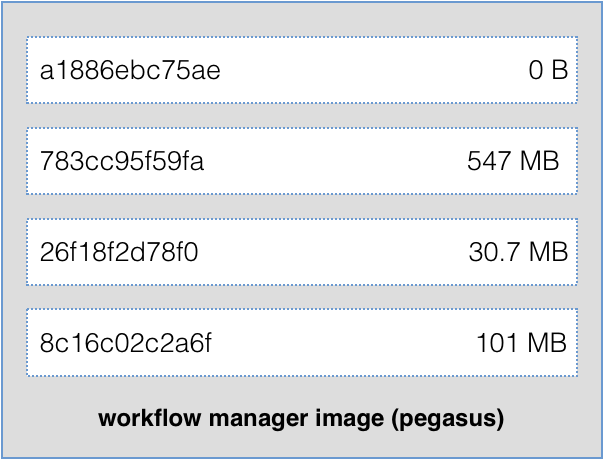
\includegraphics[width=0.6\textwidth]{Figures/docker-filesystems-multilayer}
    \caption{Representación \textit{union file system}}
    \label{fig:arquitectura}

    

\end{figure}	

    Para la definición de ordenes Docker utiliza un archivo para construir las imágenes, este archivo es Dockerfile. Cada Dockerfile es un script compuesto de  comandos y argumentos listados sucesivamente para realizar de forma automática acciones en la imagen de base para crear una nueva imagen. Esto permite simplificar el despliegue de aplicaciones desde el inicio hasta el final. \\
    
	Docker \textit{Registries} son repositorios de imágenes, estos pueden ser públicos y privados, vía a estos los usuarios pueden compartir las imágenes personalizadas o bases. Docker cuenta con un repositorio publico llamado Docker Hub, Docker Hub es un repositorio central donde se pueden compartir y obtener imágenes, estas imágenes pueden ser verificadas tanto en la autenticidad y integridad a través un firmado y verificación de datos \cite{bui2015analysis}. Los \textit{registries} son parte fundamental de eco sistema de Docker como una herramienta de desarrollo y despliegue de aplicaciones. Un caso de uso de un eco sistema típico que utiliza Docker está descrito por los siguientes eventos y la figura \ref{fig:dynamic}:
	\begin{itemize}
		\item Devs (desarrolladores) utiliza una imagen lista para usar, ya sea por ejemplo Java, PHP o Rails, está puede ser obtenida de repositorios públicos o privados.
		\item Paralelamente, ops (operaciones) pueden contribuir añadiendo patrones de seguridad o de despliegue.
		\item Devs y ops envían y traen sus cambios a través de Docker con comandos como commit, push, pull, tag hasta llegar a una versión de producción
		\item Ops traen los cambios a los servidores de producción, staging o quality assurance
	\end{itemize}
	
\begin{figure}[]
  \centering
  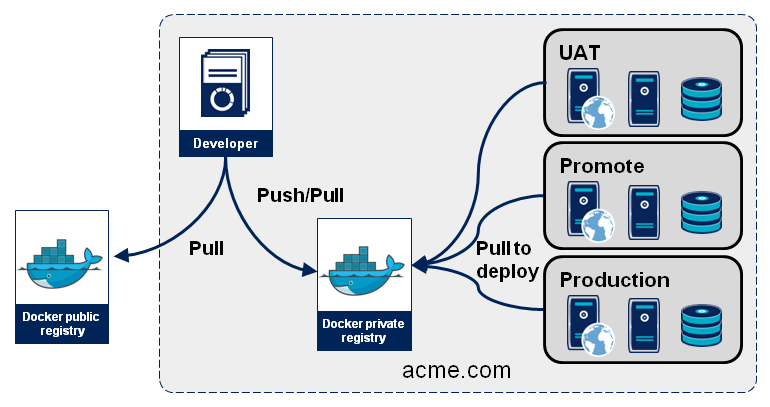
\includegraphics[width=0.6\textwidth]{Figures/registry-dynamic.png}
    \caption{Representación \textit{Dinámica de un \textit{Docker registry} }}
    \label{fig:dynamic}
\end{figure}	
	
Un Docker \textit{container} consiste de  un ambiente virtual con: sistema operativo, con archivos de usuarios y metadata, cada \textit{container} es construido a partir de una imagen como se mencionó anteriormente. Esa imagen indica a Docker lo que contiene el \textit{container} y asocia un proceso inicial, el cual es un proceso que debe correr cuando el  \textit{container} es iniciado. \cite{Docker:2015:understanding}. Para describir los pasos incluidos en la creación de un \emph{container}, se ejemplificará con la creación de uno.

\begin{verbatim}
	docker run -i -t ubuntu /bin/bash
\end{verbatim}
	\begin{itemize}
		\item \emph{Docker Client} le informa al Docker que debe correr un \emph{container}.
		\item El comando será el \textit{init 0} del container en este caso en \emph{/bin/bash}
		\item \textbf{Traer la imagen:} Docker verifica la existencia de la imagen Ubuntu y sino existe en el host, entonces Docker descarga de un \textit{registry} ya sea privado o publico. Si la imagen existe entonces crea el container.
		\item \textbf{Asignar un \emph{filesystem} y montar una capa \emph{read-write}:} El 
			\textit{container} es creado en el \emph{filesystem} y se añade una capa en modo 
			\emph{read-write} a la imagen.
		\item \textbf{Crear la red y conectar con el \emph{bridge interface}:} Crea la interfaz de red que permite que el Docker \textit{container} pueda hablar con el host a través del bridge (docker0).
		\item \textbf{Asignar un IP:} Asigna una dirección IP del pool al \textit{container}
		\item \textbf{Capturar el \emph{output}, \emph{input} y errores}.
	\end{itemize}

Docker utiliza dos funcionalidades de Linux \emph{namespaces} y \emph{cgroups} para crear ambientes virtuales para los \textit{containers}. \emph{cgroups} o \emph{control groups} proveen un mecanismo de contabilidad y limites de recursos que pueden utilizar los \textit{containers}\cite{bui2015analysis}. Los \emph{namespaces} proveen del aislamiento que es llamado \textit{container}. Cuando sea crea un \textit{container}, Docker crea un conjunto de \emph{namespaces} para el \textit{container}. Los \emph{namespaces} utilizados por Docker: mount (mnt) para el manejo del montaje, PID para el aislamiento de los procesos, net para el manejo de interfaces y IPC para acceder a recursos de IPC. 

	\subsection{Aislamiento}
	\subsubsection{A isolation}
	
	Docker logra el aislamiento de los procesos separando los procesos en \emph{namespaces} y limitando los permisos y la visibilidad de los procesos a otros \emph{containers}. \emph{PID namespaces} (añadido en el kernel \( \geq 2.6.3.2)\) es el mecanismo utilizado, logrando que un proceso que se encuentra en el container solo pueda ver procesos que se encuentra en ese container. Por lo tanto un atacante no puede observar procesos de otro container, lo que aisla al  \textit{container} este nivel \cite{bui2015analysis, LVM:2015:Online}.
	
	\subsubsection{Filesystem isolation}
	
	Docker usa \emph{mount namespaces} o \emph{filesystem namespaces} para aislar los \emph{filesystems} asociados a los containers. De la misma forma que ocurre con los procesos, los eventos del \emph{filesystem} que ocurre en el container afectan a ese container.
	Pero existen \emph{Linux kernel file systems} que deben ser montados desde host para que el container pueda funcionar correctamente, esto permite a los containers acceso directo al host. Docker utiliza dos técnicas para proteger el host: primero montar los \emph{file-systems} en modo lectura para evitar que puedan escribir en ellos y eliminar la opción de montar \emph{file-systems} en modo escritura y lectura \cite{walsh:2014:Online}.
	
	\subsubsection{Device isolation}
	Docker utiliza \emph{cgroups} que permite especificar que \emph{device} puede ser utilizado con el container. Esto bloquea la posibilidad de crear y usar \emph{device nodes} que puedan ser utilizados para atacar el host. Los \emph{device nodes} que son creados para cada container por defecto: son: /dev/console, /dev/null, /dev/zero, /dev/full, /dev/tty*, /dev/urandom, /dev/random, /dev/fuse. \cite{walsh:2014:Online}
	
	\subsubsection{IPC isolation}
	IPC (\emph{inter-process communication} es un conjunto de objetos para el intercambio de data a través de los procesos, como semáforos, colas de mensajes, segmentos de memoria compartida. Los procesos corriendo en los containers utilizan \emph{IPC namespaces} que permite la creación de un \emph{IPC} separado y independiente para cada container, con esto se previene que procesos en un container interfieran con otros containers o el host.
	
		
	\subsubsection{Network isolation}
	Para cada container, Docker crea una red independiente usando \emph{network namespaces}, compuesta de su propia IP, rutas, \emph{network devices} Esto permite que el container pueda interactuar con otro host a través de su propia interfaz.

	Por omisión, la conexión se realiza gracias al host que provee un \emph{Virtual Ethernet bridge} en la máquina host, llamado docker0 que automáticamente realiza un \emph{forward} de los paquetes entre las interfaces. Cuando Docker crea un nuevo container, esto establece una interfaz de red virtual con un nombre único que se conecta con el \emph{bridge (docker0)} y con la interfaz \emph{eth0} del container \cite{bui2015analysis}.
	
	\subsubsection{Limite de recursos}
	
	\emph{Cgroups} controlan la cantidad de recursos como CPU, memoria, \emph{disk I/O} que el container puede utilizar. A partir de esto se protege contra ataques de DoS.
	
	\subsubsection{Linux Capabilities}
	
	Los sistemas basado en Unix clasificando los procesos en dos categorías: \textit{privileged processes} (superuser o root) y  \textit{unprivileged processes}. El kernel salta la verificación de todos los permisos para los procesos privilegiados. Pero desde el kernel 2.2 los privilegios de los usuarios root o superuser se dividen en \textit{capabilities} las cuales el kernel puede activar o desactivar \cite{walsh:2014:Online}.\\
	\textit{Docker containers} corren en un kernel compartido con el host, en los containers es innecesario activar todas las \textit{capabilities} dado que las aplicaciones no las necesitan \cite{Docker:2015:Security}.



\label{sec-Docker_overview}
Docker is a technology that allows virtualizing a minimal version of an Operating System. Therefore users can run applications within it. Throughout this section, we introduce how Docker and its registry (Docker Hub) work, starting with how Docker images are created and stored in Docker Hub. 

\subsection{Docker repositories and files}

Docker builds a software image by reading a set of instructions from a Dockerfile. A Docker file is a text file that contains all commands to build a Docker image. Docker files usually have multiple lines, which are translated into image layers whereas Docker builds the image. In the build process, the command is executed sequentially, creating one layer after the other. When an image is updated or rebuilt, only modified layers (i.e., modified lines) are updated. 


\subsection{Publishing and Deploying Docker images from Docker Hub}

Docker Hub is an online registry that stores two types of public repositories, both official, and community. Official repositories contain public, verified images such as Canonical, Nginx, Red Hat, and Docker. At the same time, community repositories can be public or private and are created by any user or organization.
By using that registry and a command line, it is possible to download and deploy Docker images locally as a running container into a host executing thus the software within the image. 
Anyone has the chance to create and store images into the Docker Hub registry by first creating a descriptor file called Dockerfile. 
This descriptor describes what software packages will be within the image, builds the image and finally uploads it to Docker Hub. However, Docker Hub does not control what packages are in the images, whether the image will deploy correctly or the images might have any security problem. 
Thus, Docker images work as a black box, which refers that users know that the main software package runs within the container but they do not know the other packages needed to run it.



There are two ways of uploading images to a user repository, either by a push from a local host or automating that process from a Github repository. In order to push a repository to the Docker Hub, the users need to name their local images using their Docker Hub username, and the repository name they had created. Afterwards, users add multiple images to a repository by adding a specific \texttt{:<tag>} to it. This is all the information that normally Docker images have, being thus almost impossible to reproduce the execution environment if any of the used software packages within the images is modified. 

\section{Clair}